\documentclass[legalpaper]{article}
\usepackage[legalpaper, margin=1in]{geometry}
\usepackage[T1]{fontenc}
\usepackage[utf8]{inputenc}
\usepackage[italian]{babel}
\usepackage{graphicx}

\begin{document}
	\section{Progettazione logica}
		Lo scopo della progettazione logica è di costruire uno schema relazionale che rappresenti in modo accurato, efficiente e soprattutto correttamente tutte le informazioni descritte da uno schema ER prodotto durante la fase precedente. \\
		Questo non è una semplice trasformazione da un modello ad un altro per due motivi:
		\begin{itemize}
			\item non tutti i costrutti del modello ER possono essere tradotti nel modello relazionale;
			\item lo schema deve essere ristrutturato in modo che l'esecuzione delle operazioni avvenga il più efficientemente possibile
		\end{itemize}
		Inoltre si controllano e governano le ridondanze. Infatti per analizzarle si usano: 
		\begin{itemize}
			\item i volumi dei dati;
			\item operazioni attese;
			\item frequenza delle operazioni;
		\end{itemize}
		\'E utile dividere questo tipo di progettazione in due semplici step:
		\begin{itemize}
			\item ristrutturazione dello schema ER, basato sull'ottimizzazione e semplificazione dello schema;
			\item traduzione nel modello logico.
		\end{itemize}
		\begin{figure}[ht]
			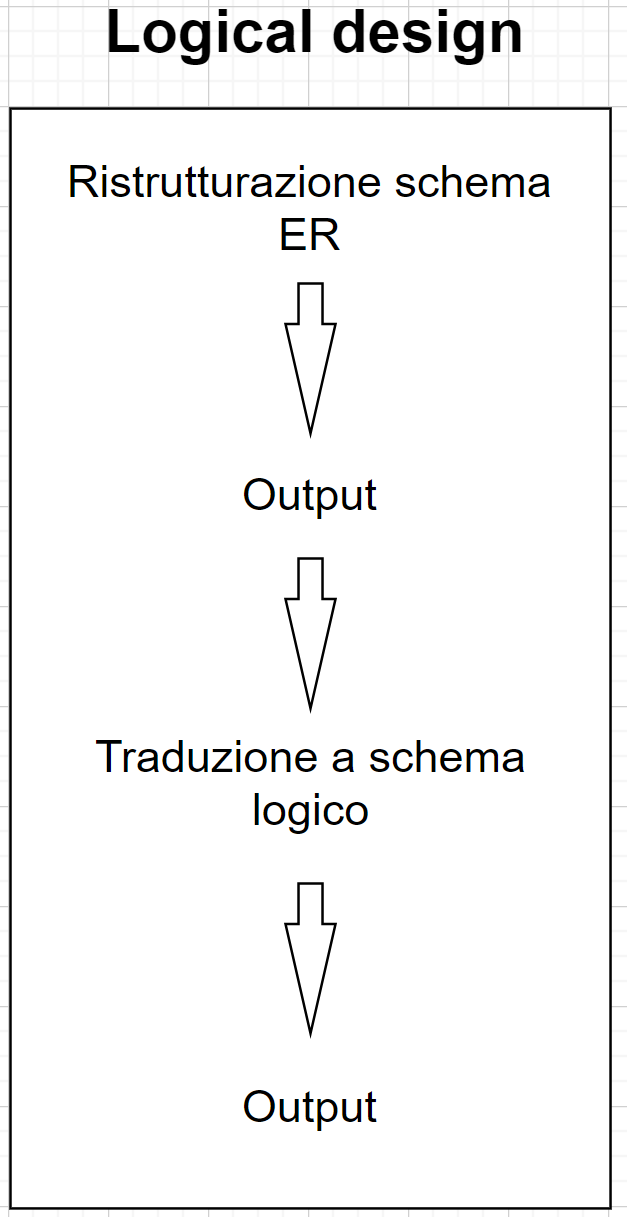
\includegraphics[width=4cm]{Schema Prog. Logica}
		\end{figure}
	\subsection{Tabella dei volumi}
		In questa sezione andiamo a definire il numero di occorrenze per ogni entità e relazione presente all'interno dello schema ER. Viene ipotizzato che i volumi facciano riferimento all'attività dopo i suoi dieci anni di vita.\\
		\newline
		\renewcommand\arraystretch{2}
		\begin{tabular}{ |p{5cm}|p{2cm}|p{5cm}| }
			\hline
			\multicolumn{3}{|c|}{\textbf{Tabella dei volumi}} \\
			\hline
			\textbf{Entità/Relazione} & \textbf{Tipo} & \textbf{Volume} \\
			\hline
			Azienda & E & 700 \\ \hline
			Ente Pubblico & E & 300 \\ \hline
			Persona Giuridica & E & 1000 \\ \hline
			Singolo Cittadino & E & 1000 \\ \hline
			Cliente & E & 2000 \\ \hline
			effettua & R & 40000 \\ \hline
			Richiesta & E & 40000 \\ \hline
			per & R & 40000 \\ \hline
			Assistenza & E & 40000 \\ \hline
			inerente & R & 40000 \\ \hline
			Guasto & E & 40000 \\ \hline
			composto da & R & 19000 \\ \hline
			Intervento & E & 19000 \\ \hline
			gestito da & R & 110 \\ \hline
			è capace di risolvere & R & 40000 \\ \hline
			Tecnico & E & 110 \\ \hline
		\end{tabular}

	
	\subsection{Tabella delle operazioni}
	Per ogni operazione indicata precedentemente, andiamo a definire la frequenza con la quale essa viene eseguita e la sua tipologia:
	\begin{itemize}
		\item \textbf{Batch}: operazioni che si possono "ignorare", ovvero vengono svolte quando il sistema non lavora in pieno regime (ad esempio tarda sera). Facendo così, si lascia spazio alle operazioni più importanti;
		\item \textbf{Interactive}: operazioni più importanti, dove la velocità di esecuzione deve essere veloce. Il tempo di risposta quindi deve essere veloce.
	\end{itemize}
		\renewcommand\arraystretch{2}
		\begin{tabular}{ |p{5cm}|p{2cm}|p{5cm}| }
			\hline
			\multicolumn{3}{|c|}{\textbf{Tabella delle operazioni}} \\
			\hline
			\textbf{Operazione} & \textbf{Tipo} & \textbf{Frequenza} \\
			\hline
			Operazione 1 & I &  19 volte a settimana \\ \hline
			Operazione 2 & I & 150 volte a settimana \\ \hline
			Operazione 3 & I & 450 a settimana \\ \hline
			Operazione 4 & B & 6 volte all'anno \\ \hline
			Operazione 5 & I & 30 volte a settimana \\ \hline
			Operazione 6 & B & 1 volta a settimana \\ \hline
			Operazione 7 & B & 1 volta al mese \\ \hline
			Operazione 8 & I & 10 volte al giorno \\ \hline
			Operazione 9 & B & 1 volta al mese \\ \hline
			Operazione 10 & B & 3 volta a settimana \\ \hline
		
		\end{tabular}	
	
	\subsection{Caso di studio (NB da inserire nel capitolo 2.4!!!!!!!!!!!!!!!!!!!)} 
	Per la realizzazione del sistema informativo è stato teorizzato un business-plan di un'azienda di piccole/medie dimensioni che opera a livello regionale.
	Consideriamo la seguente situazione dopo 10 anni di attività:
	\begin{itemize}
		\item numero clienti totale: 10000 (fedeli e non);
		\item numero tecnici totali: 75;
		\item media clienti annuali: 1000;
		\item media di 2 richieste di assistenza per cliente all'anno;
		\item media di 3 interventi per ogni assistenza richiesta;
		\item in media 300 clienti rimangono fedeli al nostro servizio;
		\textbf{NB: DEVI INSERIRE LA DEFINIZIONE DI FEDELI NELLA TABELLA DEI TERMINI !!!!!!! ---> per fedeli si intende tutti quei clienti che faranno rifermento a noi come aziende per qualsiasi guasto negli anni a venire}
	\end{itemize}
	Supponiamo che dei 10000 clienti avuti in 10 anni, 300 siano rimasti fedeli a noi. Di conseguenza l'undicesimo anno operativo dell'azienda otterrà 3000+1000=4000 clienti (fedeli + nuovi clienti annuali, fedeli e non). Facendo così, avremo 4000*2=8000 assistenze totali  e quindi ciò implica 24000 interventi.\\
	Quest'ultimi vengono divisi tra i 75 tecnici, facendo sì che ognuno di essi abbia in media 320 interventi da eseguire in un anno.\\
	Nel dodicesimo anno otteniamo un totale di 3300 clienti fedeli, arrivando a fine anno con 4300 clienti e 25800 interventi fatti, ovvero 344 a tecnico. Tutto ciò risulta essere troppo oppressivo per un lavoratore, quindi dobbiamo aumentare il numero di tecnici da assumere a fronte dell'aumento della clientela, aumentando così il volume dell'azienda stessa.\\
	Se supponiamo che ogni anno vengono assunti e/o formati 6 nuovi dipendenti, abbiamo che il rapporto interventi/tecnici rimane sempre intorno ai 320 (ovvero ogni tecnico avrà 320 interventi all'anno).\\
	Ad esempio il tredicesimo anno avremmo 87 operai con 27.600 interventi, cioè intorno ai 317 interventi per operaio.\\
	Ultimo appunto importante riguarda la distinzione che è possibile fare tra i vari clienti.
	Più in particolare del 100\% dei clienti, il 50\% risulta essere un ente pubblico mentre il restante 50\% è privato. Del 50\% pubblico, il suo 70\% fa riferimento alle aziende, mentre il 30\% agli enti pubblici.
	
	\subsection{Requisiti operazionali (NB da inserire nel capitolo 2.5!!!!!!!!!!!!!!!!!!!)}
	Le operazioni principali che prenderemo in considerazione sono:
	\begin{itemize}
		\item operazione 1: inserire un nuovo cliente -> 19 volte a settimana;
		\item operazione 2: creare una richiesta di assistenza -> 150 volte a settimana;
		\item operazione 3: creare una richiesta di intervento -> 450 volte a settimana;
		\item operazione 4: inserire un nuovo dipendente -> 6 all'anno;
		\item operazione 5: visualizzare le richieste di assistenza di uno specifico cliente -> 30 a settimana;
		\item operazione 6: visualizzare il numero di guasti per tipologia -> 1 a settimana. Questo dato può fornirci utili informazioni inerenti alle tipologie di sistemi meno affidabili; 
		\item operazione 7: visualizzare quale tecnico ha eseguito il maggior numero di interventi e la durata complessiva -> 1 volta al mese. Questo dato può essere utilizzato per vedere in quali reparti ci sono carenze di tecnici, andando così a mirare l'assunzione/training dei nuovi dipendenti;
		\item operazione 8: visualizzare lo storico degli interventi di un assistenza -> 10 volte al giorno, perchè si vuole monitorare il più possibile l'impiego dei tecnici, cioè chi è impegnato e dove;
		\item operazione 9: visualizzare il tempo complessivo degli interventi per ogni cliente -> 1 volta a settimana per i soli clienti che hanno richiesto un'assistenza nel periodo immediato;
		\item operazione 10: visualizzare gli interventi effettuati da ogni tecnico -> 3 volte a settimana;
	\end{itemize}
	
	
	
	
	
	
	
			
\end{document}